\documentclass[12pt]{article}
\usepackage{times}
\usepackage{latexsym}
\usepackage{graphicx}
\usepackage{url}
\usepackage{float}

\linespread{1}
\title{Anthropocentric Bias in Viral Genome Sequencing: Which Viruses Get Sequenced?}
\date{\today}
\author{Jacob Osborne}


\begin{document}

    \begin{titlepage}
        \begin{center}
            \vspace*{1in}
            \LARGE
            Anthropocentric Bias in Viral Genome Sequencing: Which Viruses Get Sequenced?

            \vspace*{1in}
            \large
            Jacob Osborne

            \vfill
            [DEGREE PROGRAM] \\
            Dr. Claus Wilke, Integrative Biology \\
            \today
        \end{center}
    \end{titlepage}
    
    \begin{abstract}
        PLACEHOLDER TEXT PLEASE IGNORE
    \end{abstract}

    \section{Introduction}

    The NCBI Viral Genomes database provides a large catalogue of viral genomes 
    sequenced by scientists around the world. It is the preeminent resource for
    obtaining records of viral genomes for scientific analysis.

    Yet, there is some doubt as to the extent to which the genomes catalogued
    therein can be taken as representative of viral genomes present in the
    natural world as a whole. We suspect the genomes of viruses that infect
    humans, domestic animals, and domestic plants - living things that are
    directly relevant to human life - are far more likely to be sequenced than
    the genomes of those which do not.

    The aim of this project, therefore, is to ascertain the extent of this
    anthropocentric bias in the NCBI database.

    \section{Data \& Methodology}

    The NCBI viral genomes database does not provide information on the hosts
    of the viruses it contains records on. Thankfully, the Virus-Host Database provides
    linkages between the various NCBI databases' (including the Viral Genomes
    database) records for viruses and the records for their hosts. Therefore,
    this project uses data from the Viral-Host Database instead of the NCBI viral
    genomes database directly.

    The Virus-Host Database in its entirety - 14,042 unique records - is utilized in
    this project.

    This presents a difficulty, however - the Virus-Host Database's records are
    formatted as a relationship between a single virus and a single piece of
    literature that shows at least one host for that virus, with the hosts shown
    in that literature linked by the record, rather than as a relationship between a
    virus and its hosts.

    As such, the database was reformatted to a custom format, each entry providing
    a one-to-many relationship between a virus and its hosts.


    %\section{Methodology}
    
    %Data obtained from the Virus-Host Database was reformatted into a "one Virus
    %to many Hosts" format using a python script, the code for which is presented
    %in the Appendix. \\
    %From this data, a breakdown of the clades to which host species present in the
    %database belonged. Further, a breakdown of the number of viruses which infect
    %species of each clade was also obtained.

    \section{Preliminary Analysis}

   
    \begin{figure}[H]
        \begin{center}
            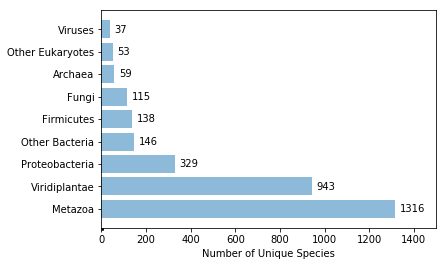
\includegraphics[width=100mm]{host_clades_figure.png}
            \caption{A breakdown of the kingdoms to which host species present in
            the database belong.}
            \label{host_clades_figure}
        \end{center}
    \end{figure}
    \begin{figure}[H]
        \begin{center}
            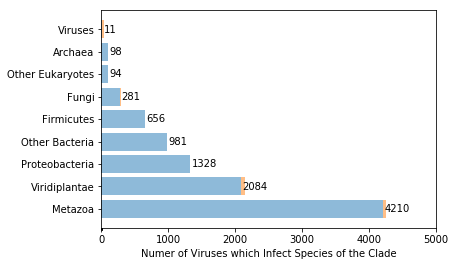
\includegraphics[width=100mm]{infects_clades_figure.png}
            \caption{A breakdown of viruses capable of infecting species of
            the given kingdom. The orange part represents viruses which can
            infect species of multiple kingdoms.}
            \label{infects_clades_figure}
        \end{center}
    \end{figure}

    Figure \ref{host_clades_figure} shows the vast majority of host species in
    the database are either animals (Metazoa) or plants (Viridiplantae). Fungal
    host species are relatively uncommon in the data.

    We see a similar pattern in the number of virus species that find their
    hosts in a given clade, as shown in Figure \ref{infects_clades_figure}.
    The numbers there are roughly proportional to those in Figure
    \ref{host_clades_figure}, save that plants seem to make up a somewhat
    proportionately smaller portion of the data. It also shows that viruses
    which are capable of infecting species belonging to more than one distinct
    kingdom are extremely rare in the data set; thus, we can effectively ignore
    this overlap.

    These figures show a very small number of fungal species and fungal viruses
    present in the database. While there are a number of domesticated species of
    fungus, and a comparison involving these and their wild counterparts may
    prove useful to this investigation, this relatively small degree of data
    on the subject resulted in our decision to exclude fungal species and their
    viruses from the rest of the investigation, and focus solely on plants and
    animals.

    \section{Results}

    \begin{figure}[H]
        \begin{center}
            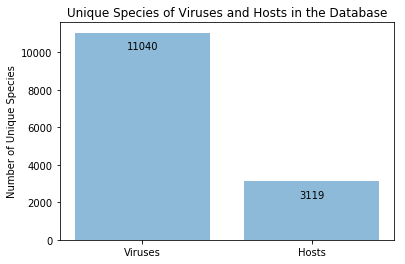
\includegraphics[width=100mm]{unique_species_figure.png}
            \caption{A comparison of the number of unique species of virus and of
            host present in the database.}
            \label{unique_species_figure}
        \end{center}
    \end{figure}

    As shown in Figure \ref{unique_species_figure}, there are just under 3
    times as many unique species of virus as of host. This means we can expect,
    for each host species in the database, multiple species of virus that infect
    it.

    This is not entirely the case, however. An examination of the distribution of
    the data, shown in Figure \ref{viruses_per_host_figure}, shows an enormous skew
    towards the lower end in the number of viruses per host species. In particular,
    well over half of the host species in the database - 1,797 species, to be exact -
    have only a single documented virus in the database.
    
    \begin{figure}[H]
        \begin{center}
            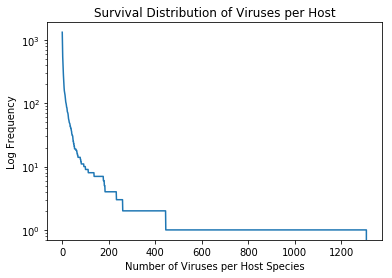
\includegraphics[width=100mm]{viruses_per_host_figure.png}
            \caption{The distribution of the number of unique species of virus
            capable of infecting each host species included in the database.}
            \label {viruses_per_host_figure}
        \end{center}
    \end{figure}

    It is almost certainly not the case that these species play host to only a
    single species of virus. This indicates certain species are far, far more likely
    to have their viruses examined and sequenced.

    Unsurprisingly, the host species with by far the largest number of
    sequenced viruses - 1,309 distinct species - is \emph{Homo sapiens}. However,
    the next most common host are rather surprising: two strains of 
    \emph{Mycolicibacterium smegmatis} - MC2 115 and one left unlabeled - with a
    combined 680 unique species of virus preying on them.

    \begin{table}[H]
        \begin{tabular}{|l||c|}
        \hline
        Host species                                 & \# of Viruses \\ \hline\hline
        \textit{Homo sapiens}                        & 1,309         \\ \hline
        \textit{Mycolicibacterium smegmatis MC2 155} & 446           \\ \hline
        \textit{Solanum Lycopersicum} (Tomato)       & 261           \\ \hline
        \textit{Mycolicibacterium smegmatis}         & 234           \\ \hline
        \textit{Escheria coli}                       & 185           \\ \hline
        \textit{Bos taurus} (Cattle)                 & 182           \\ \hline
        \textit{Sus scrofa} (Pig)                    & 178           \\ \hline
        \textit{Mus musculus} (House mouse)          & 138           \\ \hline
        \textit{Pseudomonas aeruginosa}              & 113           \\ \hline
        \textit{Staphylococcus aureus}               & 101           \\ \hline    
        \end{tabular}
        \caption{The ten most common host species in the database.}
        \label{most_common_hosts_table}
    \end{table}

    As shown in Table \ref{most_common_hosts_table}, species with the largest
    numbers of viruses seemed to be a mix of domesticated species (both plants
    and animals) and an assortment of bacteria. The reason for the predominance of
    \emph{Escheria coli}, \emph{Pseudomonas aeruginosa}, and \emph{Staphylococcus
    aureus} seems obvious: all three are relatively common, potentially pathogenic
    bacteria species, with \emph{E. coli} in particular being a model organism for
    bacterial study in general. It therefore stands to reason they would be a
    particular focus of phage research.

    The predominance of \emph{Mycolicibacterium smegmatis} is more curious, as the
    bacterial species is not of any especial relevance. However, an examination of 
    its entries in the database reveals a possible reason why - nearly every virus
    attributed to it in the database is listed as being a phage of Mycobacteria in
    general [CITE]. The Mycobacterium clade includes numerous species of pathogenic
    bacteria, including those responsible for tuberculosis and leprosy [CITE]. As 
    phage therapy has been a major focus in research for treatments for these
    diseases in recent years, it therefore becomes clear that
    \emph{Mycolicibacterium smegmatis}'s predominance in the database is a result
    of its use as a model organism for Mycobacterium phage research.
    

\end{document}